%!TEX root = ../../Heun_Dale_Haney_A_dynamic_approach_to_input_output_modeling.tex
%%%%%%%%%%%%%%%%%%%%% chapter.tex %%%%%%%%%%%%%%%%%%%%%%%%%%%%%%%%%
%
% sample chapter
%
% Use this file as a template for your own input.
%
%%%%%%%%%%%%%%%%%%%%%%%% Springer-Verlag %%%%%%%%%%%%%%%%%%%%%%%%%%
%\motto{Use the template \emph{chapter.tex} to style the various elements of your chapter content.}
\motto{We try to measure what we value. 
We come to value what we measure.~\emph{\cite[p.~2]{Meadows:1998aa}}

\hfill---\emph{Donella Meadows}}

%%%%%%%%%%%%%%%%%%%%%%%%%%%%%%%%%
%%%%%%%%%% Value Flows %%%%%%%%%%
%%%%%%%%%%%%%%%%%%%%%%%%%%%%%%%%%
\chapter{Value flows}
\label{chap:value} % Always give a unique label
% use \chaptermark{}
% to alter or adjust the chapter heading in the running head
\chaptermark{Value}
%%%%%%%%%%%%%%%%%%%%%%%%%%%%%%%%%
%%%%%%%%%%%%%%%%%%%%%%%%%%%%%%%%%
%%%%%%%%%%%%%%%%%%%%%%%%%%%%%%%%%




%% \abstract{Each chapter should be preceded by an abstract (10--15 lines long) that summarizes the content. The abstract will appear \textit{online} at \url{www.SpringerLink.com} and be available with unrestricted access. This allows unregistered users to read the abstract as a teaser for the complete chapter. As a general rule the abstracts will not appear in the printed version of your book unless it is the style of your particular book or that of the series to which your book belongs.\newline\indent
%% Please use the 'starred' version of the new Springer \texttt{abstract} command for typesetting the text of the online abstracts (cf. source file of this chapter template \texttt{abstract}) and include them with the source files of your manuscript. Use the plain \texttt{abstract} command if the abstract is also to appear in the printed version of the book.}

%% Use the template \emph{chapter.tex} together with the Springer document class SVMono (monograph-type books) or SVMult (edited books) to style the various elements of your chapter content in the Springer layout.


\abstract*{In this chapter, we develop techniques to account for flows of economic value
through economies.
We employ the prevailing subjective theory of value for our framework.
Value accounting equations were developed and applied to example
economies~A--C. % chktex 8
We noted the need for terms that describe creation and destruction
of value within economic sectors.
Finally, we explored value flows 
to and from the US auto economy
and found that, in contrast to direct and emboded energy, 
there is no lack of data on value flows to and from the US auto industry.}



In Chapters~\ref{chap:direct_energy} and~\ref{chap:embodied_energy}, 
we noted that energy is the currency of Thermodynamics,
and we developed accounting equations for flows of 
direct ($\dot{E}$) and embodied ($\dot{B}$) energy through an economy.
In this chapter, we develop a framework for accounting
value flows\index{economic value!flow of} ($\dot{X}$) through economies.
Accounting flows of value is a necessary step along
the path to developing equations (in Chapter~\ref{chap:intensity}) 
that describe the energy intensity of intermediate
and final products within an economy.


%%%%%%%%%% Methodology %%%%%%%%%%
\section{Methodology}
\label{sec:Value_Methodology}
%%%%%%%%%%


We begin by explicitly describing what we mean by value. 
We follow the standard, neoclassical approach 
of using the market price at the time of an exchange
to determine the value of the flows of products (goods, services and capital). 
As materials and energy flow in one direction between sectors, 
currency flows in the opposite direction. 
The monetary flow is an easy and logical
proxy for the value of the material and energy flows. 
Market transactions are readily captured and the data 
to estimate these flows is available in most countries. 
(See for example, \url{http://www.iioa.org/io-data/io-data.html}) 
Using the price at the time of exchange to place a value 
on the flow of material goods and resources 
assumes a \emph{subjective} theory of value. 
Value is subjective in that it is based on a price 
that two trading partners are willing to accept 
for any subjective reason. 
Value is based on the agreement of a fair price 
by the human trading partners. 
The market price (and, by the subjective theory of value, the value) 
is not a measure of any \emph{intrinsic}
value of the goods (e.g., for bio-diversity or ecosystem services). 
Market prices ignore the costs and benefits that accrue 
to other parties (externalities), 
including the impact of trade on the quality of human relations, 
just distribution of resources, 
or sustainable scale of the economy.\cite[p.~55]{Daly1996} (***CITE Daly, Herman E., Beyond Growth, 
Boston: Beacon Press, 1996, p. 55)   
Section~\ref{sec:theory of value} 
contains further discussion of the benefits and limitations 
of the neoclassical subjective theory of value. 

Market prices also ignore any inherent value 
in the physical flows
of materials and energy to and from the biosphere.\footnote{Flows 
	of value between the economy and the biosphere
	are conspicuously absent 
	from the figures in this chapter. 
	(See, for example, Figure~\ref{fig:basic_value}.)}
Although it would be nice to ascribe monetary value to material flows between
the economy and the biosphere, it is very challenging to do so.
****ADD CITE (Nordhaus, William, The Future of Environmental and Augmented
National Accounts
An Overview, Survey of Current Business, November 1999, p. 45-65.  \url{http://www.bea.gov/scb/account_articles/national/1199od/nordhaus.htm}.) ***ADD CITE (United Nations, et al., Environmental-Economic Accounting 2012: Experimental Ecosystem Accounting, United Nations, 2013.  (\url{http://unstats.un.org/unsd/envaccounting/eea_white_cover.pdf}) 
However, an international experimental system 
for accounting environmental and economic flows is in place.\footnote{As of this printing, 
the System of Environmental-Economic Accounting (SEEA) is in its third revision 
using a process of global consultation.}\cite{UNSEEA:aa}
If and when the challenge of ascribing value
to material resource, energy, and waste flows 
to and from the biosphere is addressed, 
our framework will be able to incorporate those values easily.  

It is important to be clear that 
despite our focus on material and energy flows through an economy, 
our framework does not assume, nor does it lead to, 
an energy theory of value.
And, our pragmatic use of the subjective theory of value
does not indicate an endorsement. 
Rather, we accept the subjective theory of value
despite several weaknesses.
Our framework values goods and services at their market prices.

Because the basic unit of analysis in our framework is the economic sector, 
flows of value within the economy are based on the prices agreed 
upon in the transactions. 
The flows of value that accompany the material and energy flows in and out 
of one sector in an economy are depicted in Figure~\ref{fig:basic_value}. 

\begin{figure}[!ht]
\centering
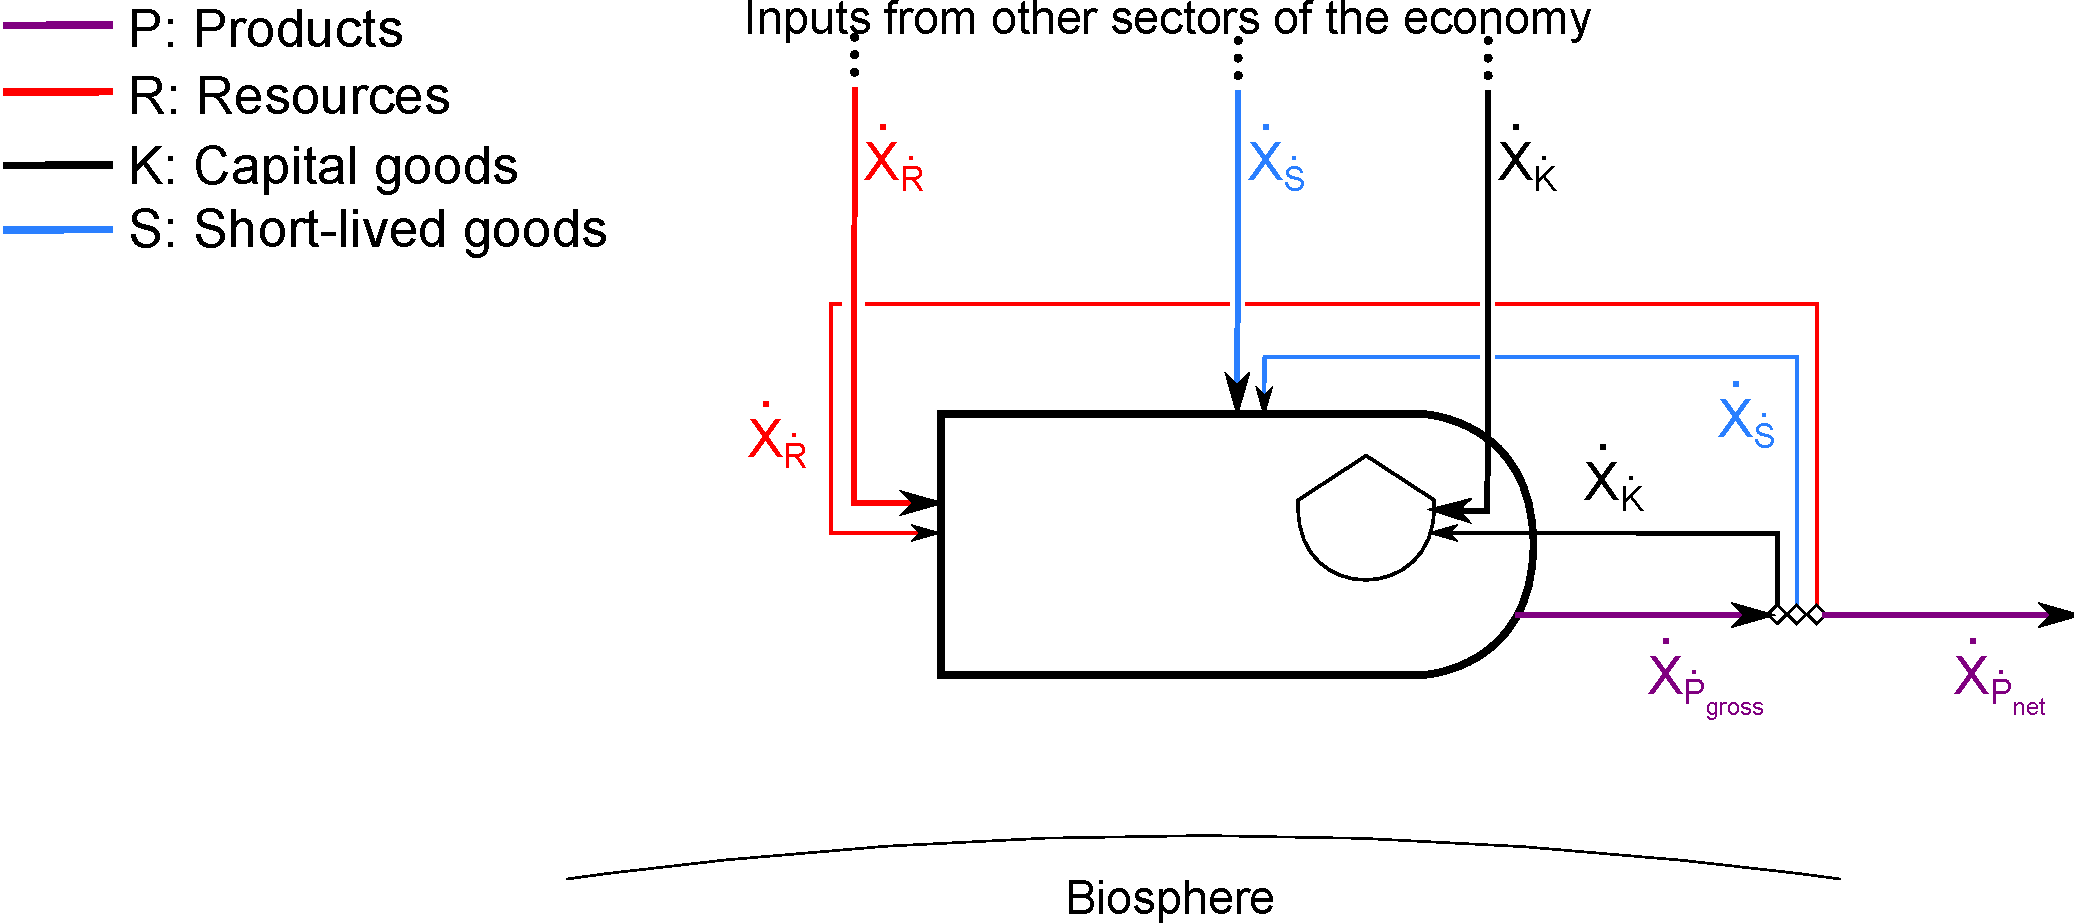
\includegraphics[width=0.8\linewidth]{Part_2/Chapter_Values/images/PERKS_basic_unit_value_all.pdf}
\caption[Flows of value for a single sector]{Flows of value ($\dot{X}$) 
for a single sector. 
The value flows are associated with each of the different 
material and energy flows outlined in previous chapters.}
\label{fig:basic_value} 
\end{figure}

We denote creation and destruction
of value within a sector using the notion of ``source'' and ``sink.''
In Figure~\ref{fig:basic_value_aggregated}, the open circle, 
``source,'' inside the economic sector represents the value-added,
that is, the value that is created by the economic processes within that sector. 
The flows of value from a value-source are denoted $\dot{X}_{gen}$. 
Similarly, black circles represent the value ``sinks''  where value is destroyed 
by economic  processes or natural disasters. 
The flows of value into the value sinks are denoted $\dot{X}_{dest}$. 
Although we do not define 
the value creation and destruction processes any further (mathematically), 
we discuss what is meant by the
underlying processes in more detail below.

\begin{figure}[!ht]
\centering
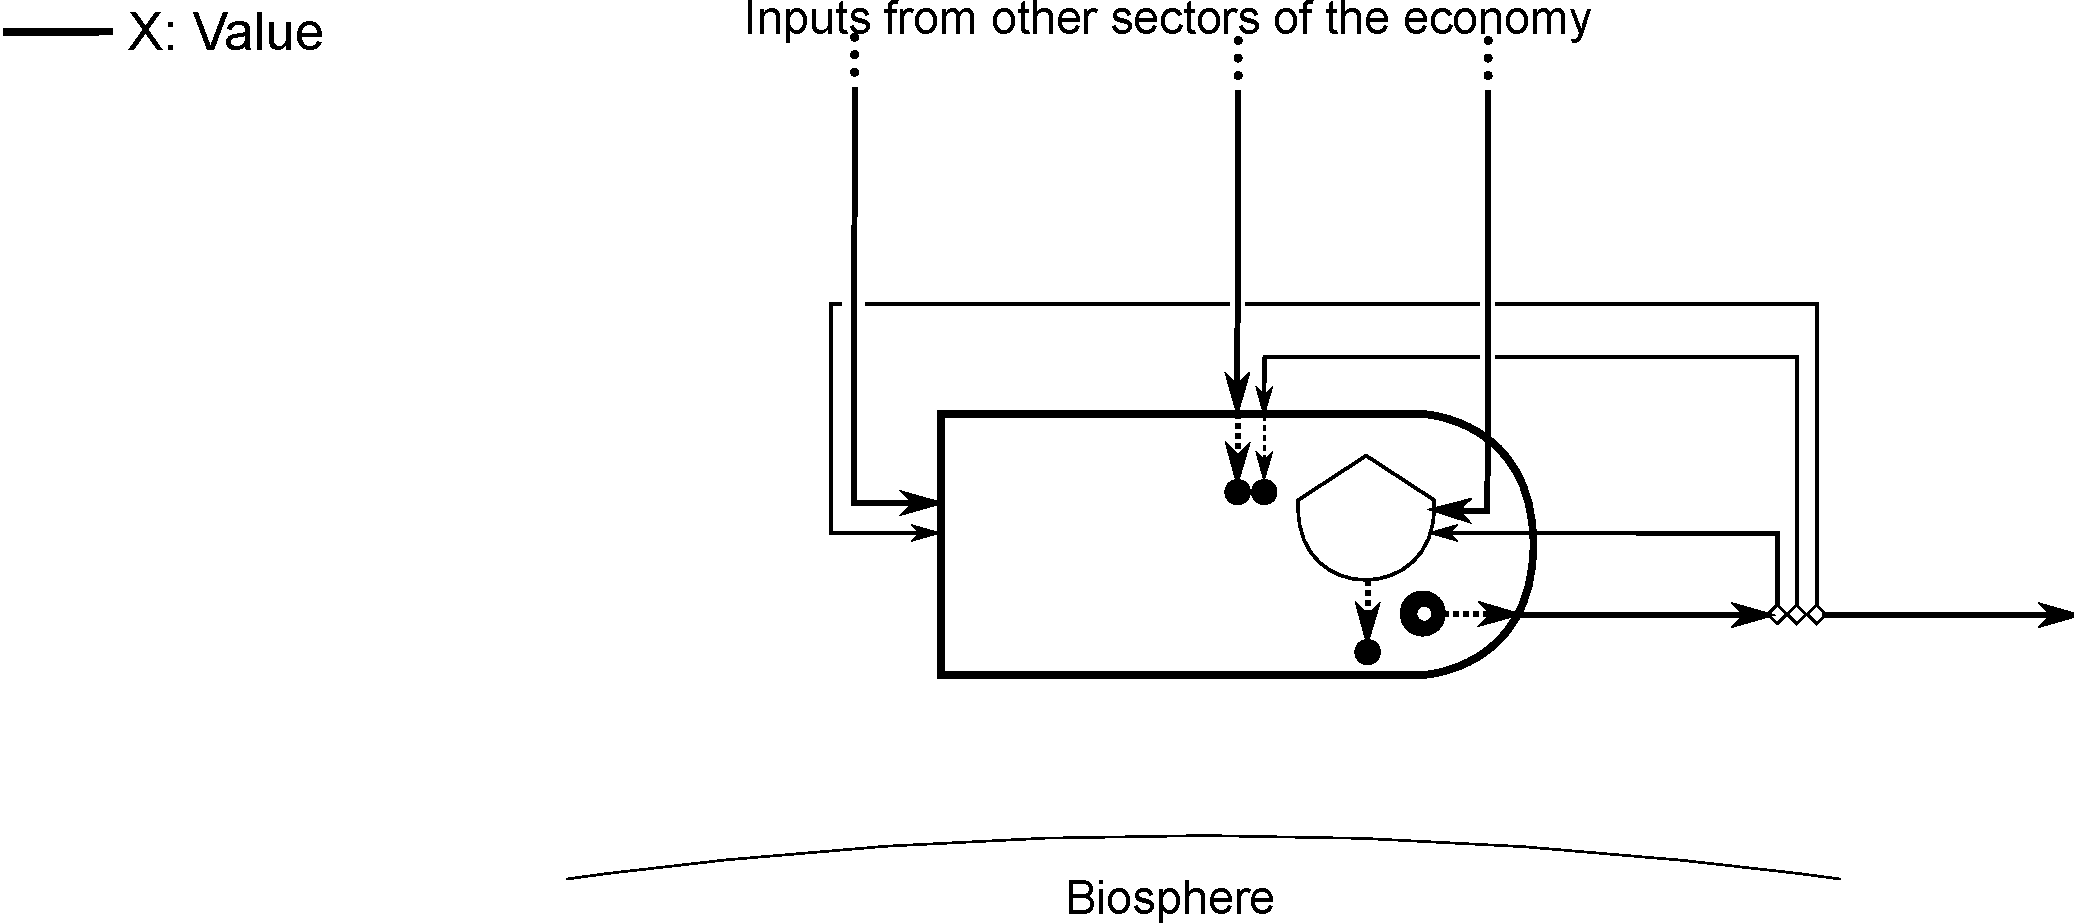
\includegraphics[width=0.8\linewidth]{Part_2/Chapter_Values/images/PERKS_basic_unit_value.pdf}
\caption[Aggregated flows of value for a single sector]{Aggregated flows of value ($\dot{X}$) 
for a single sector. 
Distinction is made between value flows that 
enter the sector and are accumulated (i.e.\ capital goods) 
and value flows that are not accumulated. 
Within the sector there is destruction of value $\dot{X}_{dest}$, 
represented by the downward arrow flowing 
into the black sink and generation of value, 
represented by the arrow flowing out of a source. }
\label{fig:basic_value_aggregated} 
\end{figure}


%%%%%%%%%% Example A: single-sector economy %%%%%%%%%%
\section{Example A: single-sector economy} % chktex 13
\label{sec:value_example_A}
%%%%%%%%%%

Figure~\ref{fig:A_value} shows flows of value in the single-sector economy.
Following typical assumptions in economic modeling, 
the economy is \emph{completely isolated} from the biosphere
in terms of both material inputs and wastes.
In other words, the value flows of an economy are \emph{independent from}
material inputs and wastes.
Value flows are independent from material inputs,
because raw materials have no economic value 
until they have been removed from the biosphere by the extraction industry.
Value flows are independent from wastes,
because wastes, by definition, have no economic value 
after they leave the economy.

\begin{figure}[!ht]
\centering
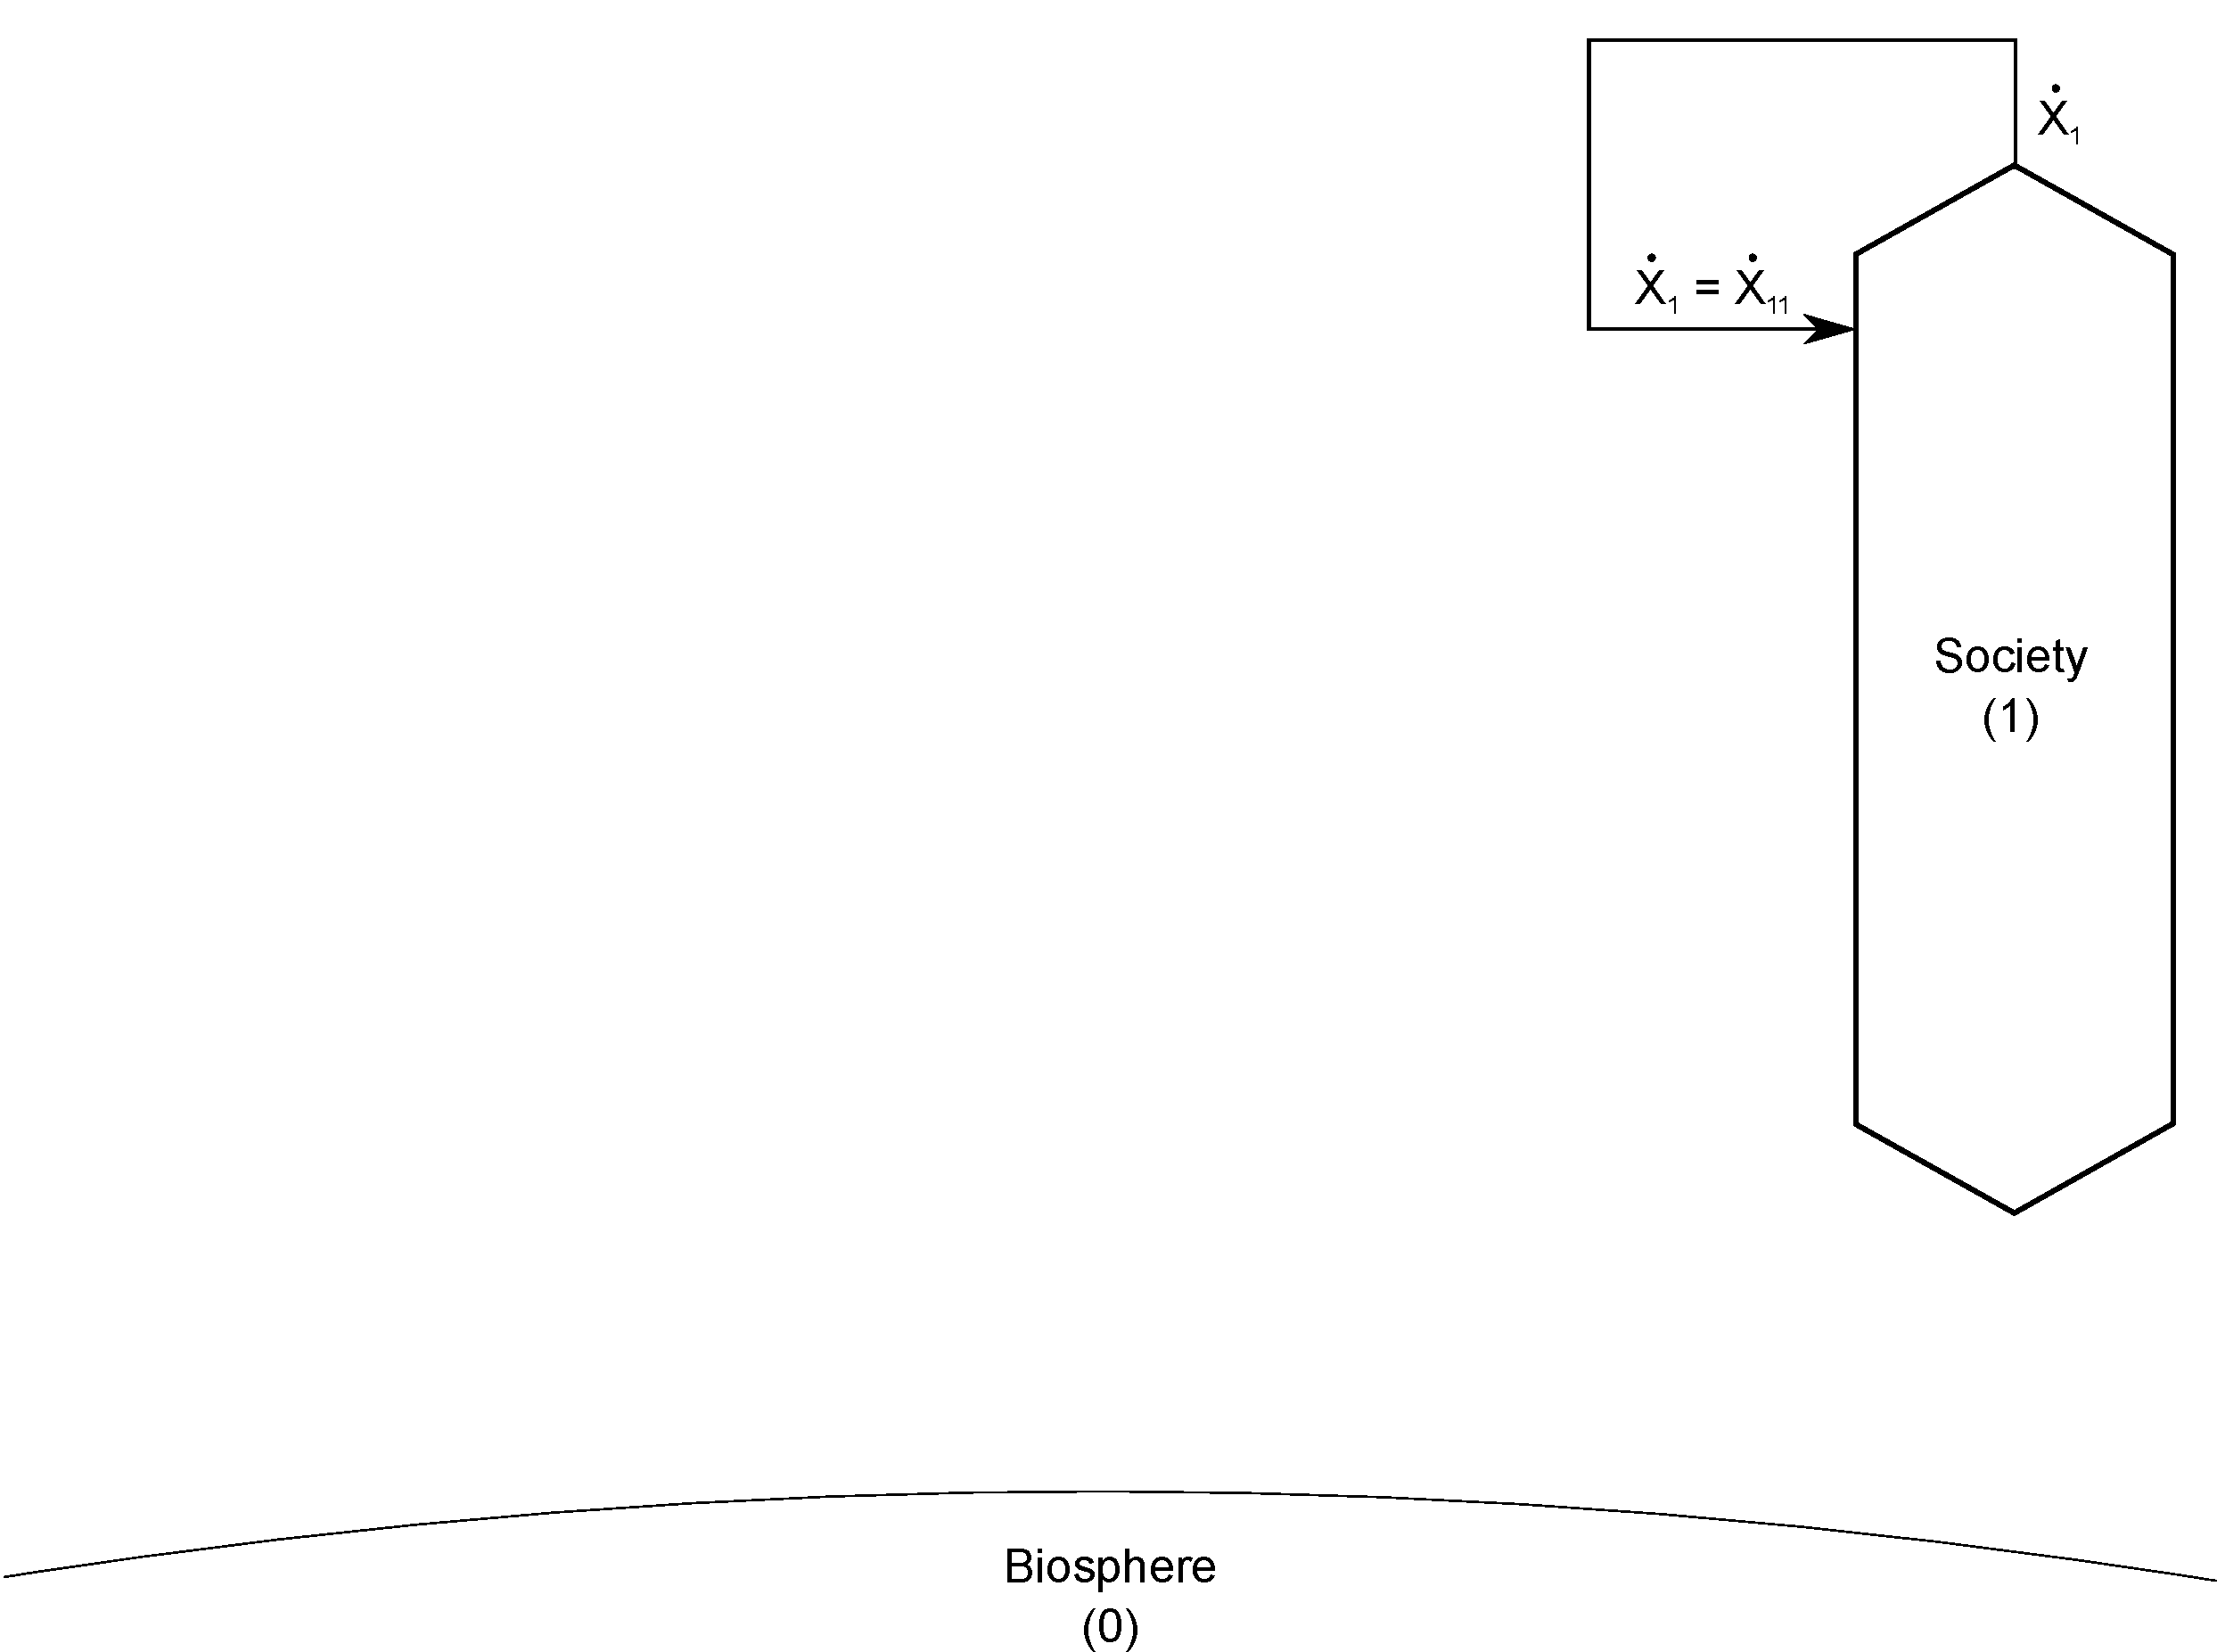
\includegraphics[width=0.8\linewidth]{Part_2/Chapter_Values/images/1_sector_value.pdf}
\caption[Flows of value for a one-sector economy]{Flows of value ($\dot{X}$) for a one-sector economy.}
\label{fig:A_value} 
\end{figure}

The contrast between Figures~\ref{fig:A_materials} and~\ref{fig:A_energy}, 
on the one hand, 
and Figure~\ref{fig:A_value}, 
on the other, is striking.  
The picture of material and energy flows in 
Figures~\ref{fig:A_materials} and~\ref{fig:A_energy} 
indicates interaction with and dependence upon the biosphere 
that is not reflected in the value flows of Figure~\ref{fig:A_value}.
The isloation of the value flows from the biosphere is a consequence
of the subjective theory of value\index{theory of value!subjective} 
that underpins modern economics.
The biosphere is akin to a third party with no voice 
in determining the value of a transaction:
it is neither buyer nor seller. 

Equation~\ref{eq:A_X_acct_1} describes the accumulation 
of value\index{economic value!accumulation}
($X$)\nomenclature[X]{$X$}{stock of economic value [\$]} in Society (1).

\begin{equation} \label{eq:A_X_acct_1}
	\frac{\mathrm{d}X_{1}}{\mathrm{d}t} 
	= \dot{X}_{11} 
	- \dot{X}_{1}
	+ \dot{X}_{gen,1}
	- \dot{X}_{dest,1}.
\end{equation}
\nomenclature[X]{$\dot{X}$}{economic value flow rate [\$/s]}
\nomenclature[Xgen]{$\dot{X}_{gen}$}{rate of generation of economic value [\$/s]}
\nomenclature[Xdest]{$\dot{X}_{dest}$}{rate of destruction of economic value [\$/s]}

\noindent{} The following subsections discuss the terms in Equation~\ref{eq:A_X_acct_1}.


%+++++++++ Example A: Economic Transactions ++++++++++
\subsection{Economic transactions ($\dot{X}_{11}$ and $\dot{X}_{1}$)}
%+++++++++

The returning arrow in Figure~\ref{fig:A_value} 
represents transactions between 
\begin{itemize}
	\item{buyers (who receive things of value, $\dot{X}_{11}$,
	in exchange for currency) and}
	\item{sellers (who give up things of value, $\dot{X}_{1}$,
	in exchange for currency).}
\end{itemize}

It is interesting to note that when a good is sold for more
than the producer paid for its inputs, 
the seller has created value and sold it into the economy. 
As a consequence, the seller's stock of currency grows,
providing the seller with an increased level of claim 
on value in the economy.

The subjective theory of value\index{theory of value!subjective}
(Section~\ref{sec:Value_Methodology})
posits that buyers and sellers agree on value at the 
time of the transaction.
Thus, $\dot{X}_{1} = \dot{X}_{11}$, and Equation~\ref{eq:A_X_acct_1}
simplifies to

\begin{equation} \label{eq:A_X_acct_2}	
	\frac{\mathrm{d}X_{1}}{\mathrm{d}t}	
	= \dot{X}_{gen,1}
	- \dot{X}_{dest,1},
\end{equation}

\noindent{}indicating that value accumulates in the economy
$\left( \frac{\mathrm{d}X_{1}}{\mathrm{d}t} \right)$
due to value generation ($\dot{X}_{gen,1}$) 
and destruction ($\dot{X}_{dest,1}$) processes only.


%+++++++++ Example A: value generation ++++++++++
\subsection{Value generation ($\dot{X}_{gen}$)}
%+++++++++

\noindent In Equation~\ref{eq:A_X_acct_1}, 
the value generation term ($\dot{X}_{gen}$) is akin to growing apples
in Section~\ref{sec:Materials_Methodology}: 
value is generated, seemingly out of nothing.
But, in fact, value is not created out of nothing. 
Rather, value is created from a variety of factors that have no apparent 
monetary cost to producers, including:

\begin{itemize}
	\item{flow of solar energy\index{solar energy}\index{energy!solar|see{solar energy}}
	into the economy,
	as in the example of growing apples,}
	\item{extraction of resources (e.g., water\index{water}, minerals\index{minerals}, and
	fossil fuels\index{fossil fuels}) or any other unpriced goods from the biosphere,}
	\item{exploitation of the unpriced waste assimilation capacity of the biosphere,}
	\item{utilization of capital stock, labor, and energy to produce products
	that are more valuable than inputs, and}
	\item{application of human ingenuity\index{ingenuity!human} 
	and innovation\index{innovation}, 
	which lead to increasingly efficient production processes.}
\end{itemize}

\noindent{}The subjective theory of value indicates that 
there is no economic value associated with these ``transactions''
that generate value, because no currency is exchanged. 

The above factors indicate that the process of value generation
has both direct and indirect impacts on the biosphere.
The direct impacts are obvious: 
extraction of non-renewable resources from the biosphere, 
at rates greater than their natural accretion,
represents unsustainable overuse of natural capital.
The indirect impacts are less obvious: 
human ingenuity can lead to increased wealth,
leading to increased demand rates for goods and services, 
whose production requires ever-increasing rates 
of unsustainable natural resource extraction.

$\dot{X}_{gen}$ is accounted as ``value added'' to an industry in national accounts.
It is calculated as the difference between gross economic output of the industry
and the cost of its intermediate inputs.~\cite{BEAVA}  ****ADD CITE BEAVA \url{http://www.bea.gov/faq/index.cfm?faq_id=184} A simple way to think of value added is
the increase in value of the raw materials from the work performed 
on them by workers and manufactured capital.


%+++++++++ Example A: value destruction ++++++++++
\subsection{Value destruction ($\dot{X}_{dest}$)}
%+++++++++

\noindent In Equation~\ref{eq:A_X_acct_1}, 
the value destruction term ($\dot{X}_{dest}$)\index{economic value!destruction of} 
is akin to consuming apples: 
value is destroyed by a process that consumes, 
or otherwise renders unusable, 
previously-valuable things in the economy
(see Section~\ref{sec:Materials_Methodology}).
The factors that lead to value destruction
($\dot{X}_{dest}$) include:

\begin{itemize}
	\item{depreciation\index{depreciation}, usually associated with disposal of 
	materials and equipment to the biosphere at end of life and}
	\item{natural disasters, such as hurricanes and typhoons,
	that destroy equipment and property.}
\end{itemize}

$\dot{X}_{dest}$ is accounted as depreciation, or ``consumpton of fixed capital,'' to an industry in the national accounts. 
It is a monetary estimate of the physical effects on assets from ``wear and tear, obsolescence, accidental damage,
and aging.''~\cite{katz2008} ****ADD CITE Katz2008
Katz, Arnold. “Accounting for Obsolescence: An Evaluation of Current NIPA Practice.” Paper prepared for presentation at The 2008 World Congress on National Accounts for Nations  in Arlington, VA, May 12-17, 2008, May 2008.


%+++++++++ Example A: GDP and Stock of Value ++++++++++
\subsection{GDP}
%+++++++++

If Society (1) in Figure~\ref{fig:A_value} represents 
the economy of an entire country, 
$\dot{X}_{1}$ is its gross domestic product (GDP)\index{gross domestic product}
in units of \$/year. 
GDP is a flow, not a stock. 
GDP is often considered a stock, but that is incorrect. 
$X_{1}$ is a stock, akin to monetary wealth. 
$X_{1}$ is a very
narrow definition of wealth
that neglects the value of natural resources, 
the value of social captial, and any
other ``wealth'' that cannot be exchanged for money. 


%%%%%%%%%% Example B: two-sector economy %%%%%%%%%%
\section{Example B: two-sector economy} % chktex 13
%%%%%%%%%%

Figure~\ref{fig:B_value} shows flows of value ($\dot{X}$) 
within a two-sector economy. 
Again, we note the isloation of value from the biosphere.

\begin{figure}[!ht]
\centering
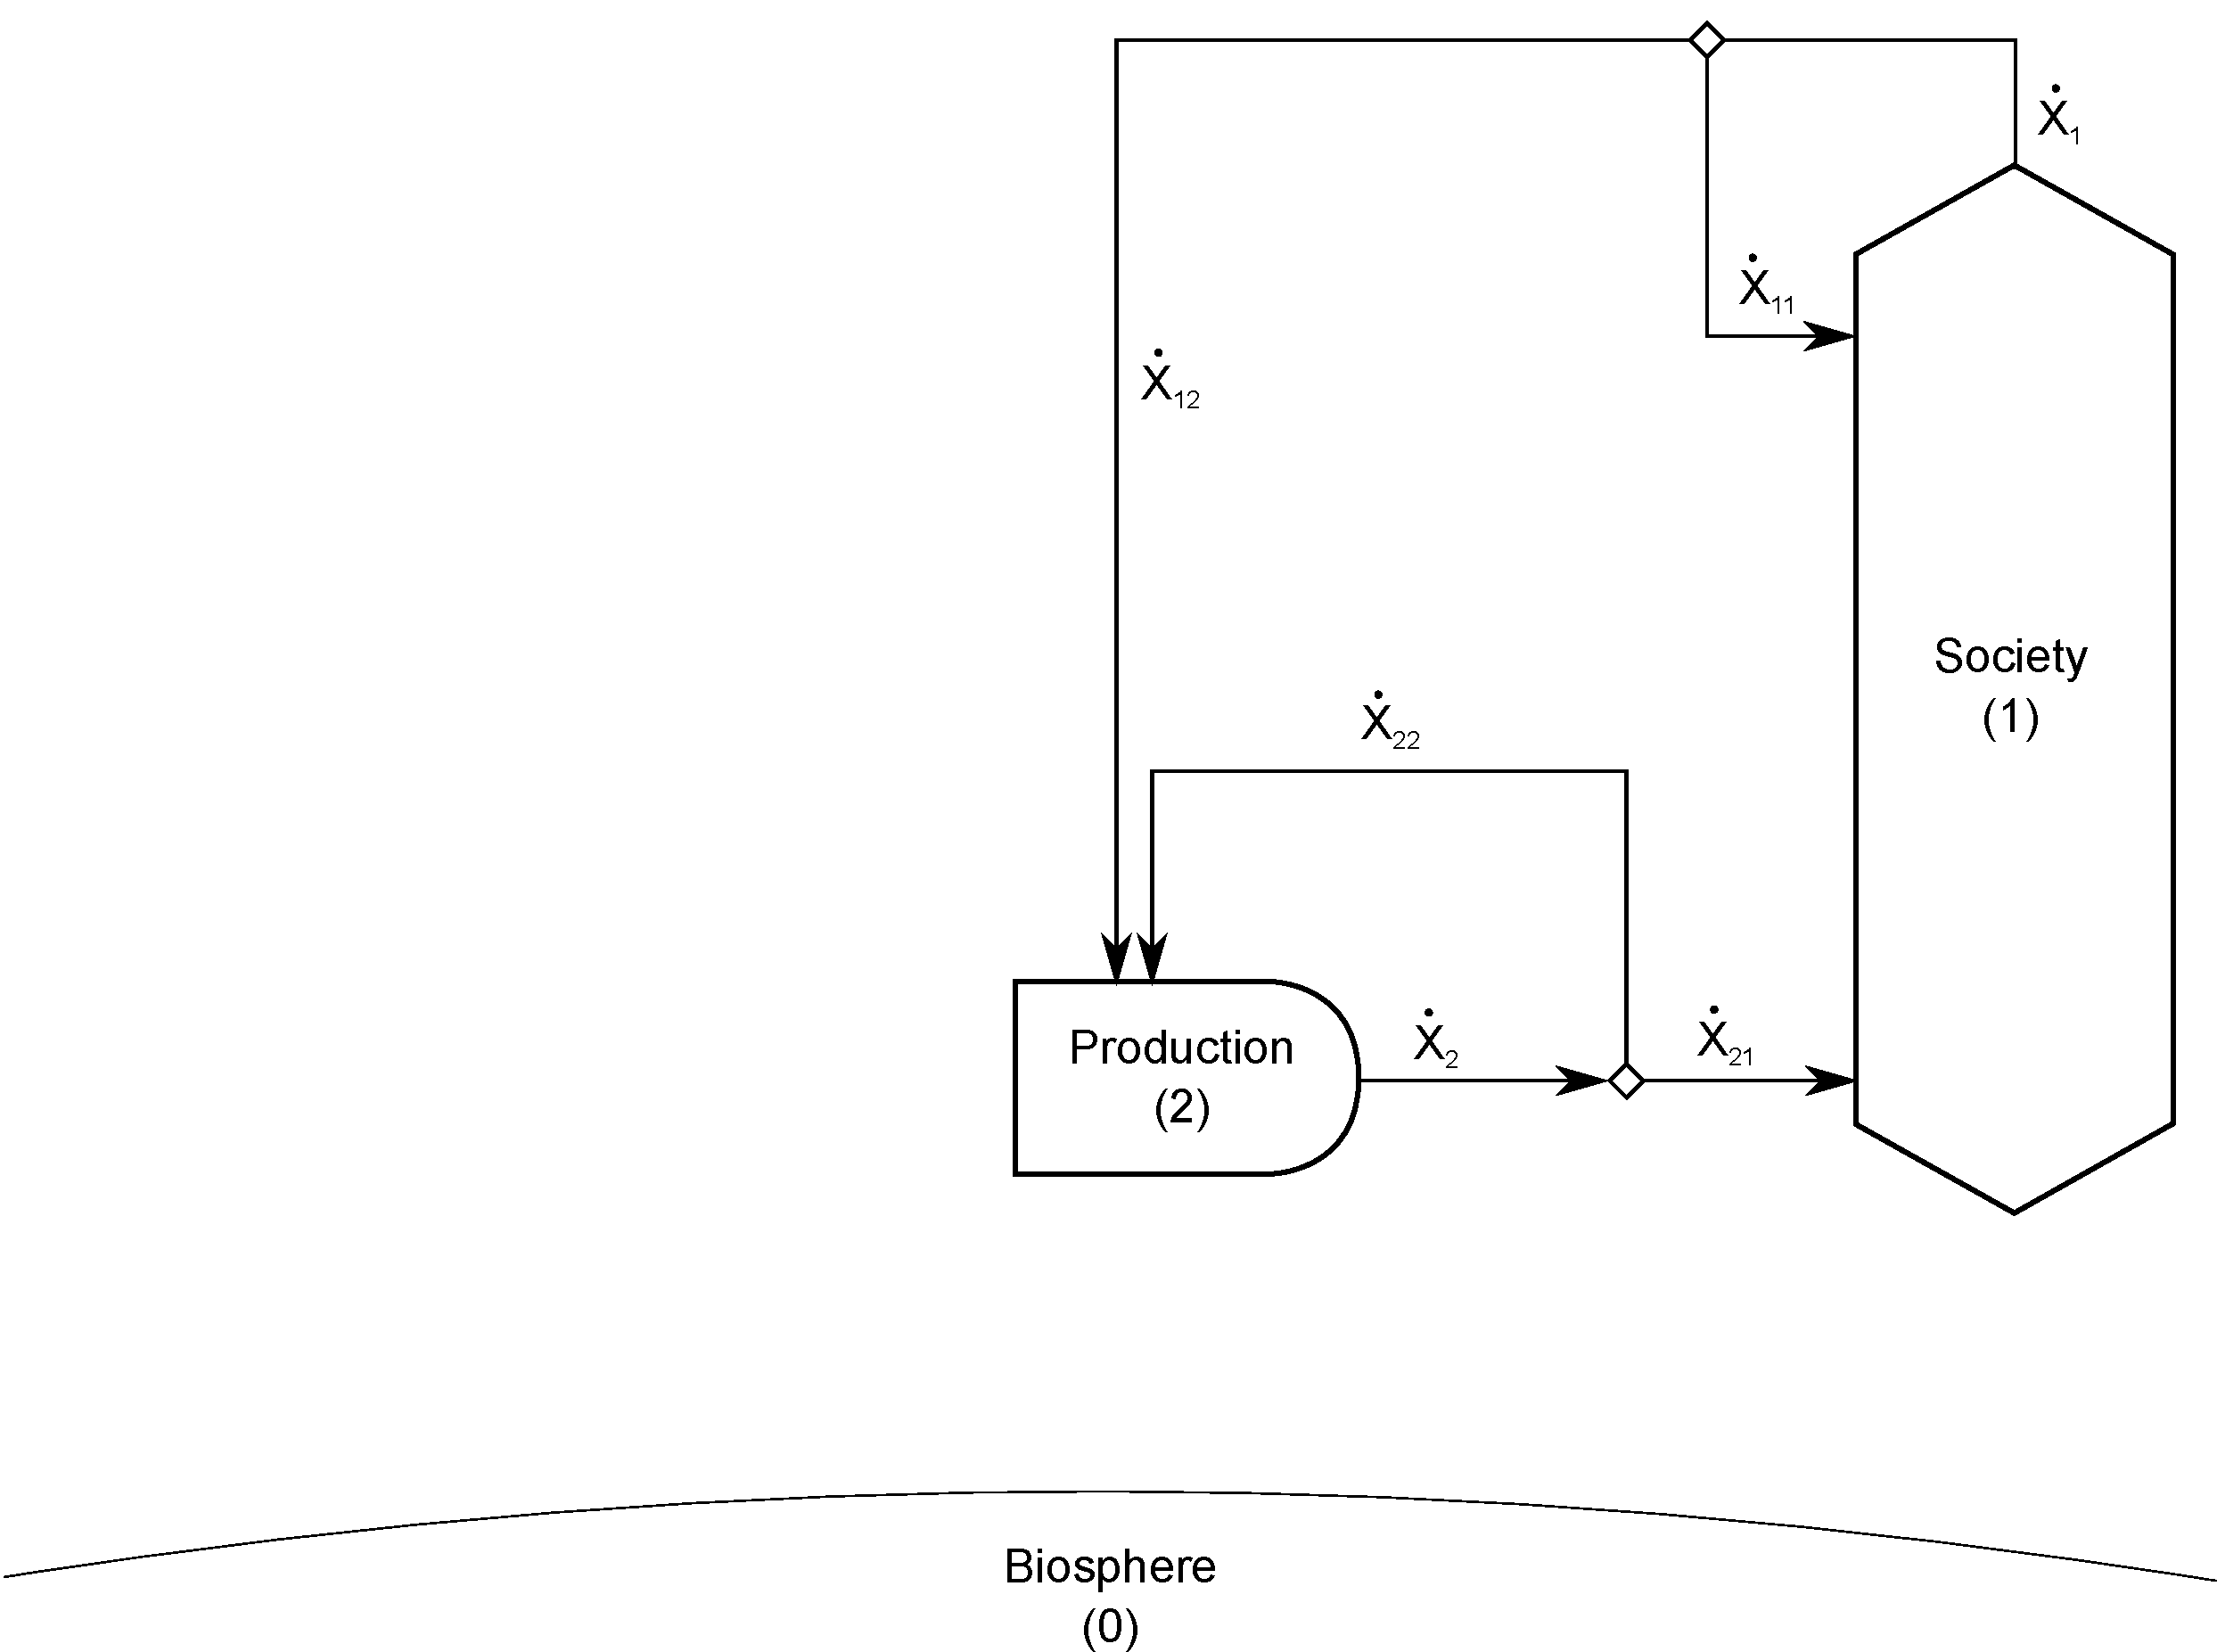
\includegraphics[width=0.8\linewidth]{Part_2/Chapter_Values/images/2_sector_value.pdf}
\caption[Flows of value within a two-sector economy]{Flows of value ($\dot{X}$) within a two-sector economy.}
\label{fig:B_value}
\end{figure}

We can account for value flows by writing
the following equations:

\begin{equation}\label{eq:B-value-1}
	\frac{\mathrm{d}X_{1}}{\mathrm{d}t}
	= \dot{X}_{11}
	+ \dot{X}_{21}
	- \dot{X}_{1}
	+ \dot{X}_{gen,1}
	- \dot{X}_{dest,1}
\end{equation}

\noindent{}and

\begin{equation}\label{eq:B-value-2}
	\frac{\mathrm{d}X_{2}}{\mathrm{d}t}
	= \dot{X}_{12}
	+ \dot{X}_{22}
	- \dot{X}_{2}
	+ \dot{X}_{gen,2}
	- \dot{X}_{dest,2}.
\end{equation}

Equations~\ref{eq:B-value-1} and~\ref{eq:B-value-2}
can be generalized as

\begin{equation}\label{eq:B-value-generalized}
	\frac{\mathrm{d}X_{j}}{\mathrm{d}t}
	= \sum\limits_{i=1}^n \dot{X}_{ij}
	- \dot{X}_{j}
	+ \dot{X}_{gen,j}
	- \dot{X}_{dest,j},
\end{equation}

\noindent{}where $n$ is the number of sectors in the economy, and $j \in [1, n]$.


%%%%%%%%%% Example C: three-sector economy %%%%%%%%%%
\section{Example C: three-sector economy} % chktex 13
\label{sec:value_example_C}
%%%%%%%%%%

Figure~\ref{fig:C_value} shows flows of value ($\dot{X}$) 
within a three-sector economy. 

\begin{figure}[!ht]
\centering
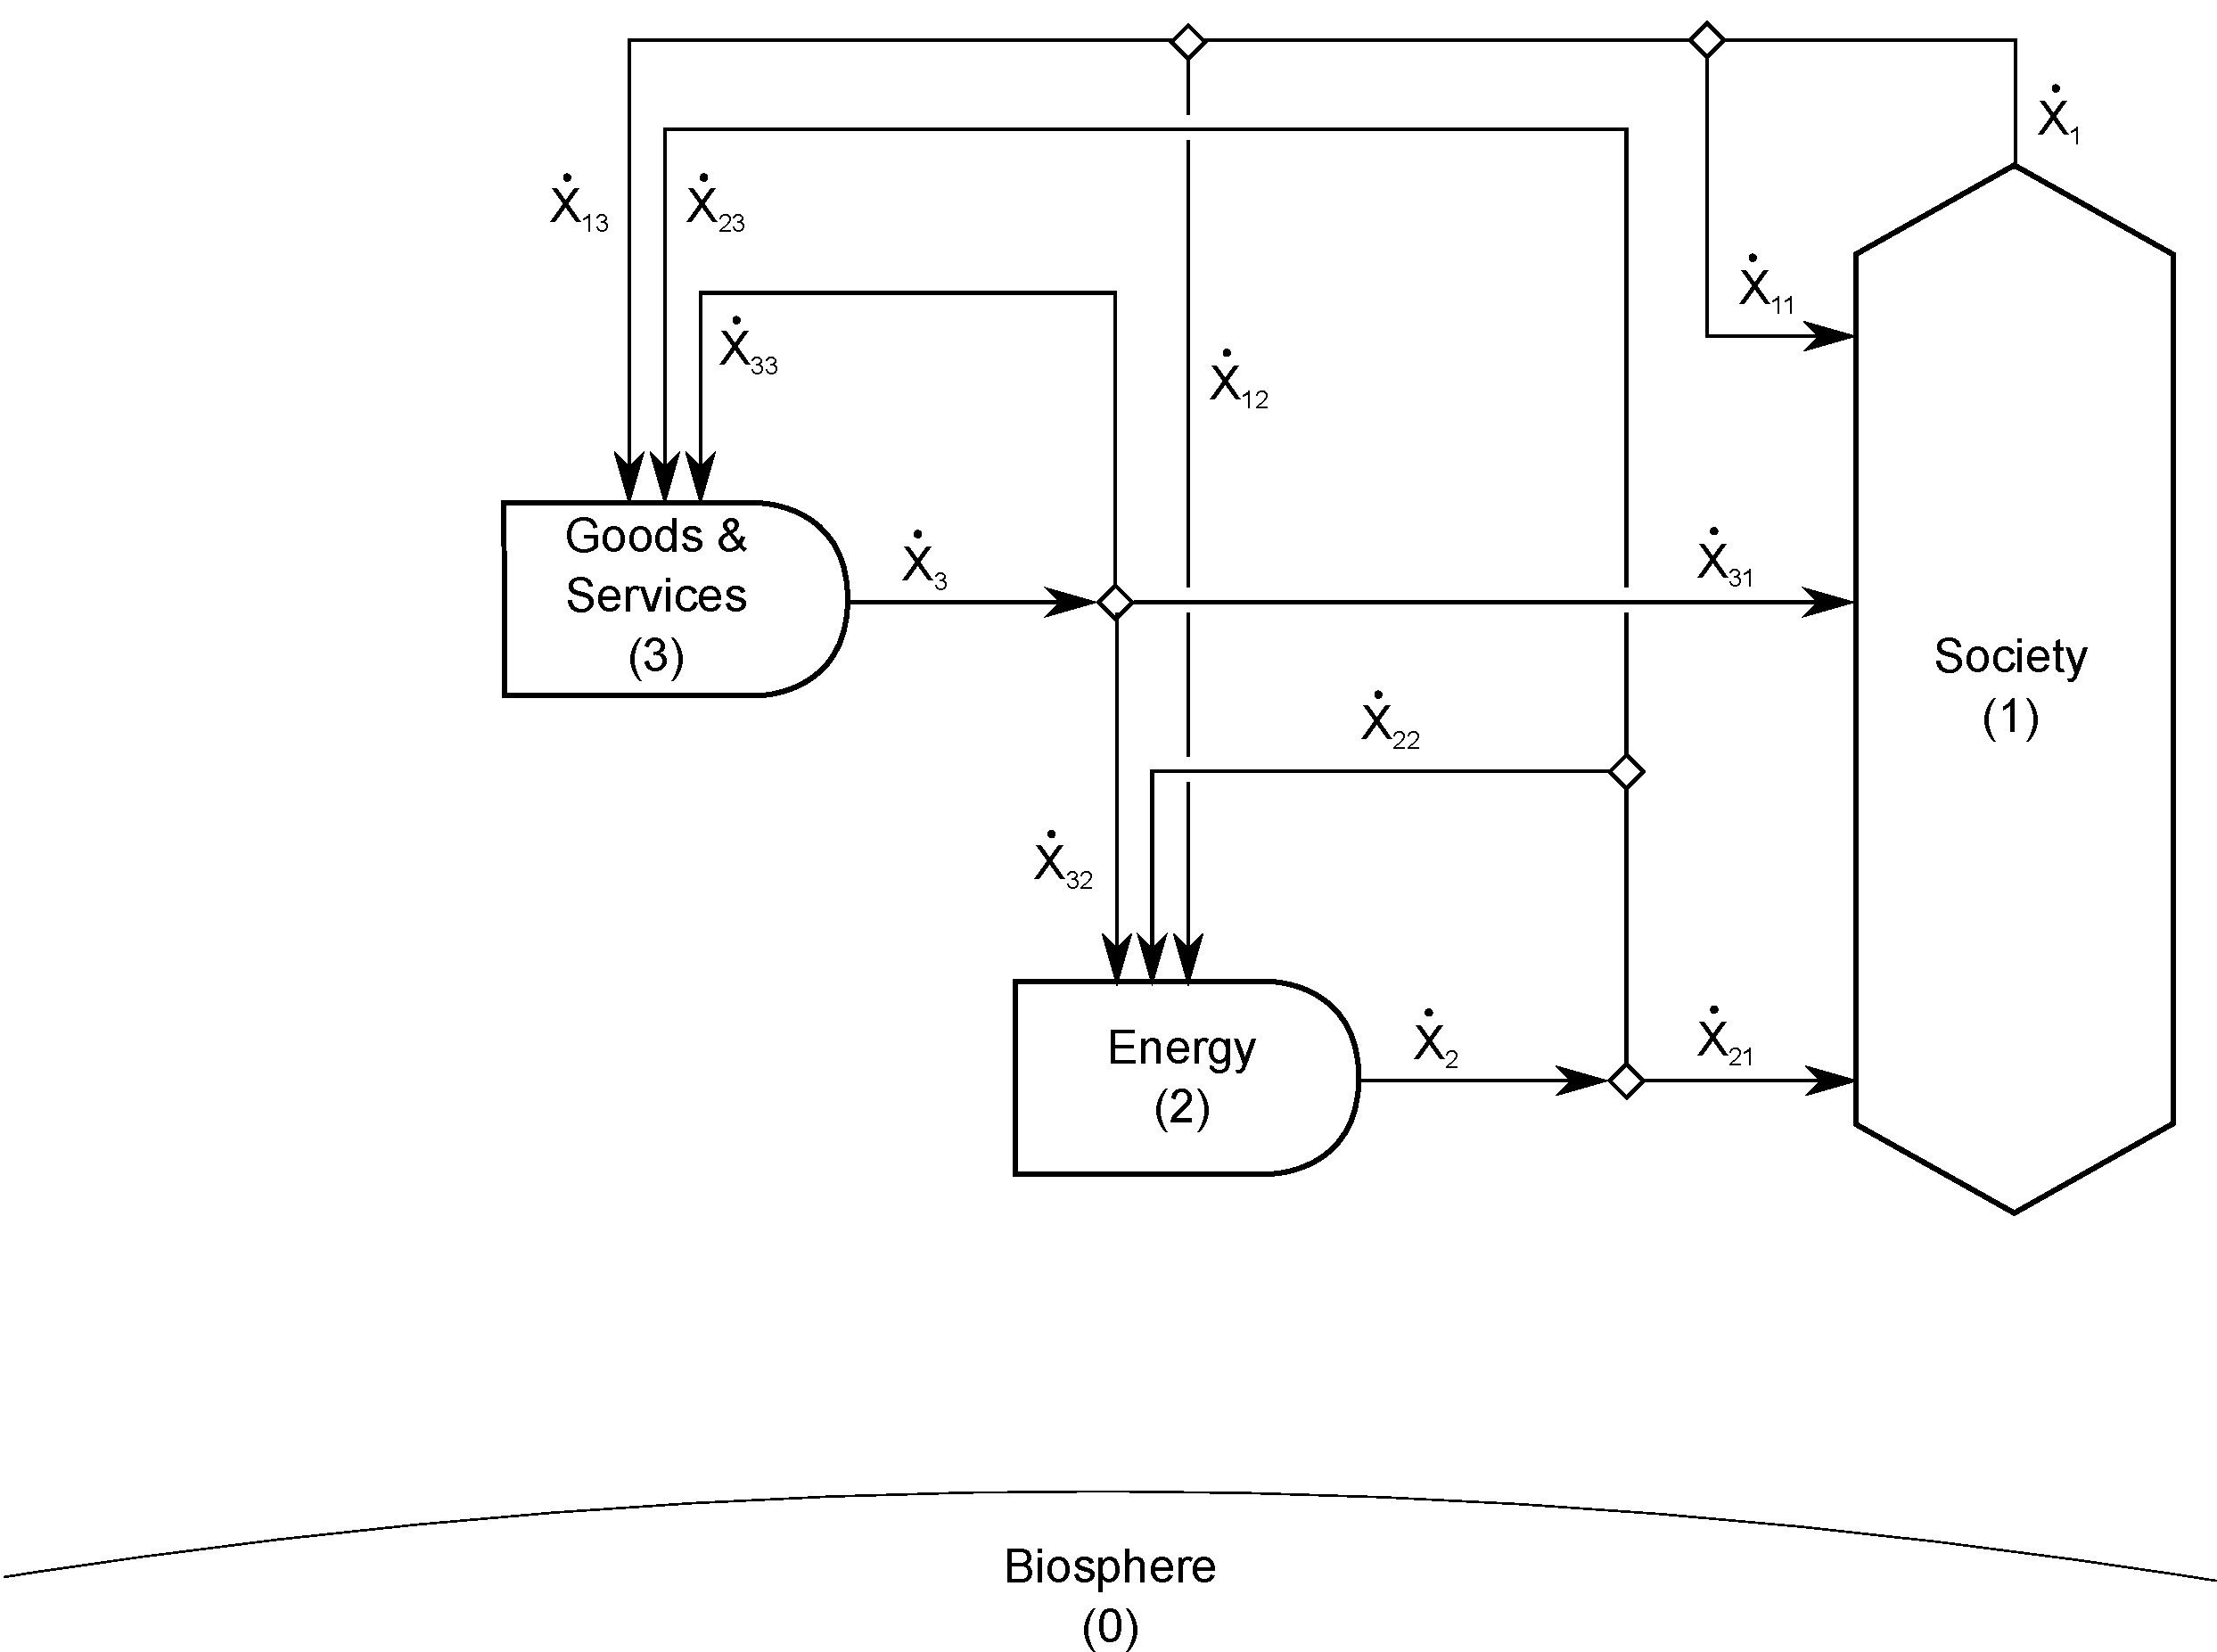
\includegraphics[width=0.8\linewidth]{Part_2/Chapter_Values/images/3_sector_value.pdf}
\caption[Flows of value within a three-sector economy]{Flows of value ($\dot{X}$) within a three-sector economy.}
\label{fig:C_value}
\end{figure}

The equations representing flows of value in Example~C are:

\begin{equation}\label{eq:C-value-generalized}
	\frac{\mathrm{d}X_{j}}{\mathrm{d}t}
	= \sum\limits_{i=1}^{n} \dot{X}_{ij}
	- \dot{X}_{j}
	+ \dot{X}_{gen,j}
	- \dot{X}_{dest,j},
\end{equation}

\noindent{}where $n$ is the number of sectors in the economy, and $j \in [1, n]$.
Equation~\ref{eq:C-value-generalized} is identical to Equation~\ref{eq:B-value-generalized}.
If we sum the value accounting equations for the entire economy, 
we obtain

\begin{equation}\label{eq:C-value-economy-a}
	\sum\limits_{j=1}^{n} \frac{\mathrm{d}X_{j}}{\mathrm{d}t}
	= \sum\limits_{j=1}^{n} \sum\limits_{i=1}^{n} \dot{X}_{ij}
	- \sum\limits_{j=1}^{n} \dot{X}_{j}
	+ \sum\limits_{j=1}^{n} \dot{X}_{gen,j}
	- \sum\limits_{j=1}^{n} \dot{X}_{dest,j}.
\end{equation}

\noindent{}With the identities

\begin{equation} \label{eq:X_identity_1}
	\dot{X}_{j}  
	= \sum\limits_{k=1}^n \dot{X}_{jk}
\end{equation}

\noindent{}and

\begin{equation} \label{eq:X_identity_2}
	\sum\limits_{j=1}^n\dot{X}_{j}  
	= \sum\limits_{j=1}^n \sum\limits_{k=1}^n \dot{X}_{jk}
	= \sum\limits_{i=1}^n \sum\limits_{k=1}^n \dot{X}_{ik}
	= \sum\limits_{i=1}^n \sum\limits_{j=1}^n \dot{X}_{ij}
	= \sum\limits_{j=1}^n \sum\limits_{i=1}^n \dot{X}_{ij},
\end{equation}

\noindent{}Equation~\ref{eq:C-value-economy-a} becomes

\begin{equation}\label{eq:C-value-economy-b}
	\sum\limits_{j=1}^{n} \frac{\mathrm{d}X_{j}}{\mathrm{d}t}
	= \sum\limits_{j=1}^{n} \dot{X}_{gen,j}
	- \sum\limits_{j=1}^{n} \dot{X}_{dest,j},
\end{equation}

\noindent{}for $j \in [1, n]$, indicating that 
value generation ($\dot{X}_{gen,j}$) 
and destruction ($\dot{X}_{dest,j}$)
are the only mechanisms by which value is accumulated or lost
$\left( \frac{\mathrm{d}X_{j}}{\mathrm{d}t} \right)$
within the economy.  This is a mathematical representation of the
value-added approach to measuring GDP. The sum of the
value-added across all industries is equivalent to the 
sum of the value of all final produced goods.~\cite{BEAValueAdded, p. 4}
****ADD CITE \url{http://bea.gov/NATIONAL/PDF/NIPA_PRIMER.PDF}


%%%%%%%%%% Value: Auto industry example %%%%%%%%%%
\section{Value in the US auto industry}
\label{sec:value_auto}
%%%%%%%%%%

To estimate value flows through the automobile industry, 
we use publicly available data from the US  Bureau of Economic Analysis (BEA)
(\url{http://www.bea.gov}).\footnote{A 
	``primer'' on using the US BEA industry data can be found on the BEA website here
	\url{http://bea.gov/industry/pdf/industry_primer.pdf}}.
The two main tables needed to estimate dynamic 
value flows and capital accumulation within the economy 
are the Input-Output Tables (I-O) and the Fixed Asset, non-residential detail, table. 
The I-O tables consist of `` make'' and use ``tables.'' 
The use table tracks which \emph{industries} (columns) 
use which \emph{commodities} (rows) 
that are made in one industry and then used in another 
as intermediate inputs ($\dot{R}$ and $\dot{S}$). 
The Use table also tracks the output that
is used for final consumption, 
including Private Fixed Investment (capital in-flows). 
However, the more detailed Fixed Asset accounts are
used to estimate all capital value flows 
in this example ($\dot{K}$) 
so that capital from other sectors can be separated 
from the capital that is produced and used within the automobile industry.  

Using these data, Figure~\ref{fig:PERKS_value_auto_ind} provides estimates 
of value flows for the US auto industry. 
Table~\ref{tab:data} contains a brief description 
of the data sources that were used 
to obtain the values in Figure~\ref{fig:PERKS_value_auto_ind}. 
Appendix~\ref{chap:auto_value_flows} contains the
detailed calculations and describes the BEA data sources.

\begin{figure}[!ht]
\centering
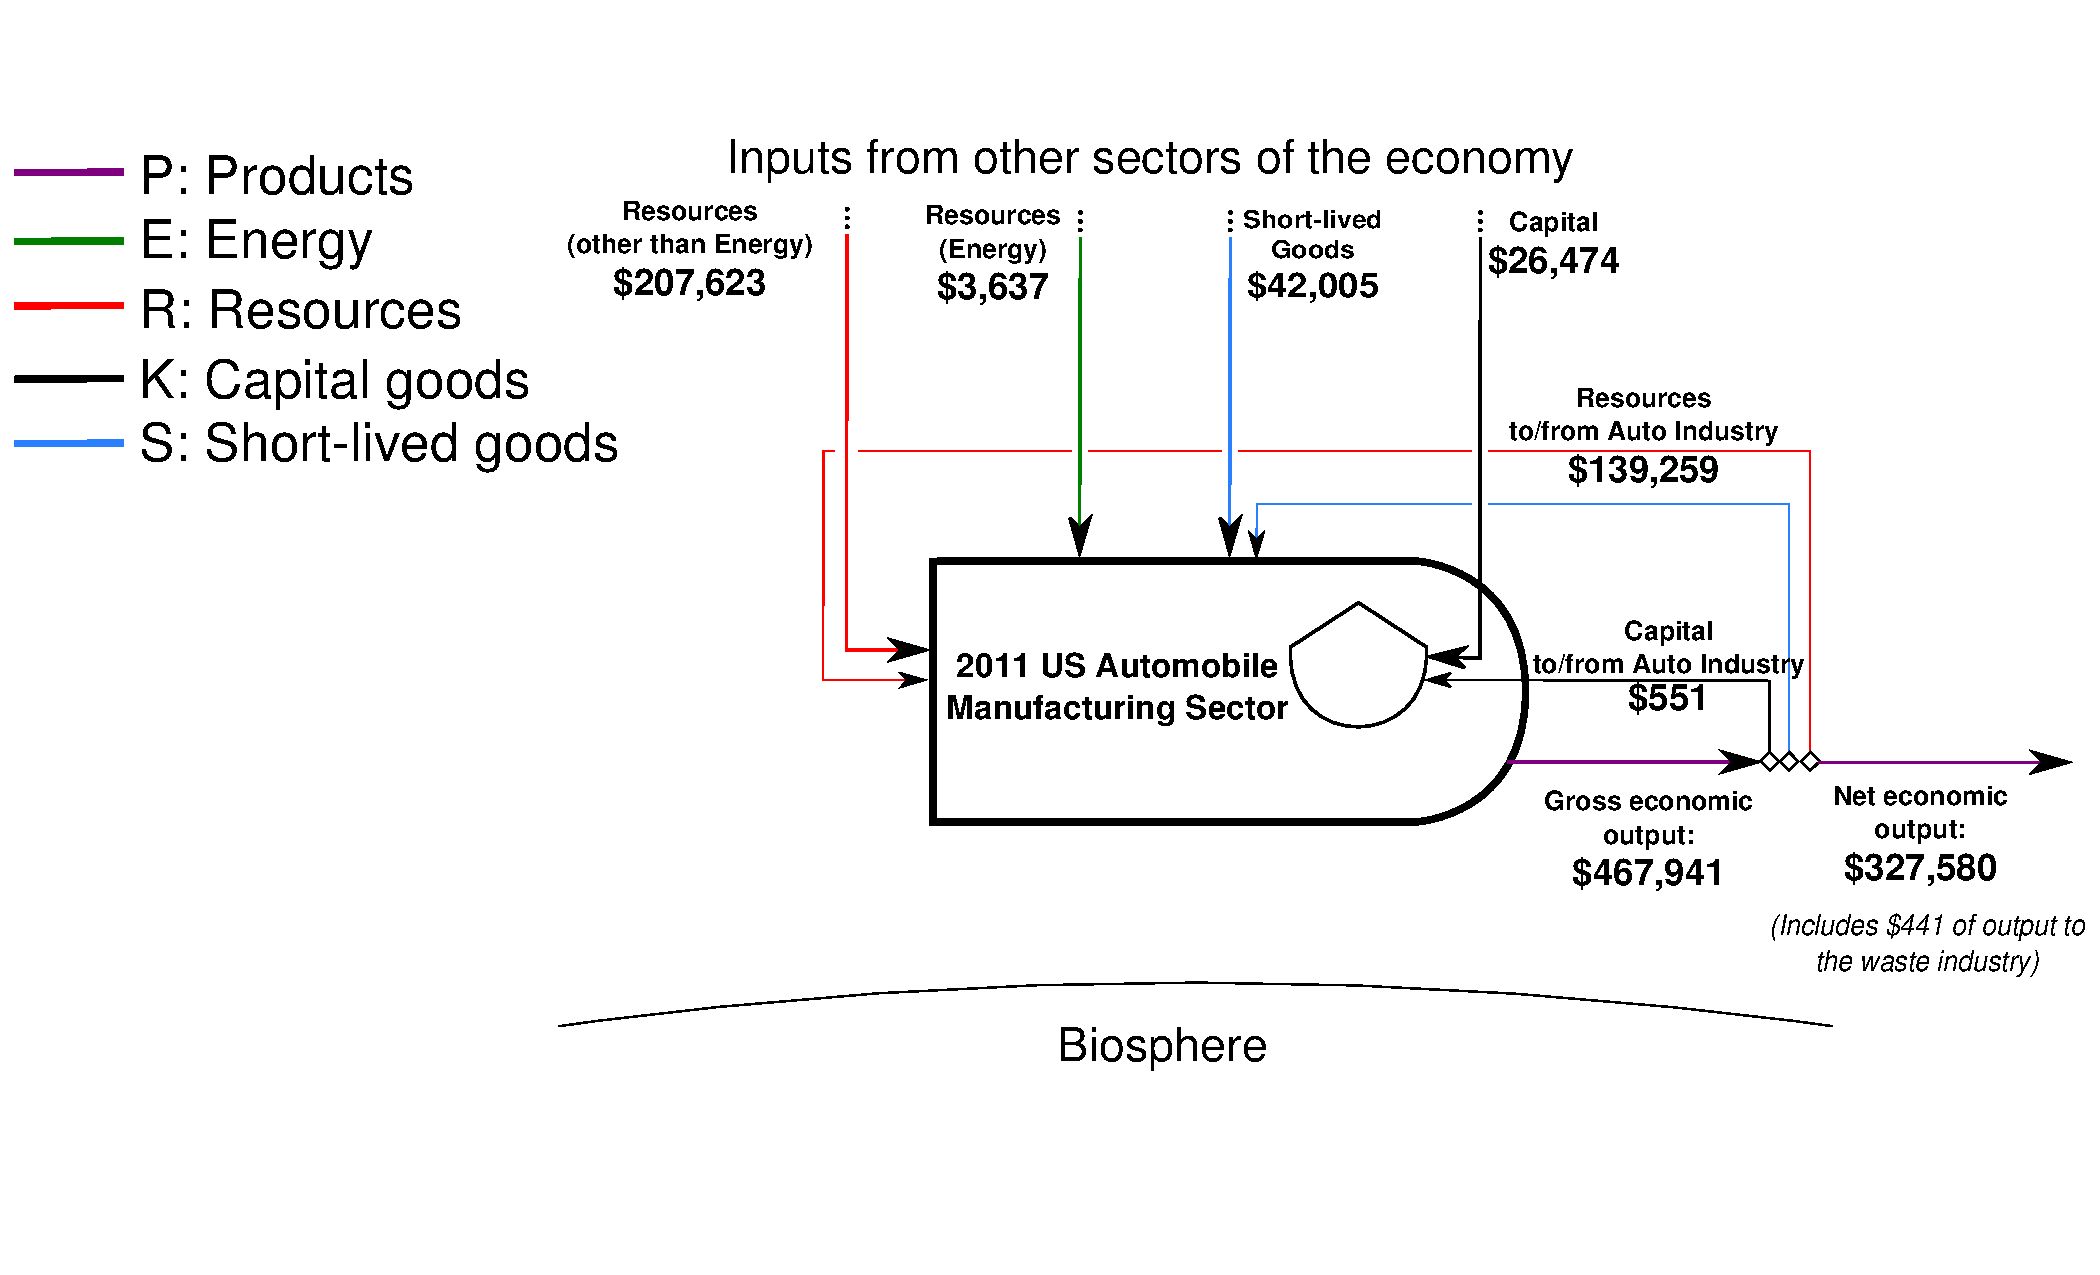
\includegraphics[width=1.0\linewidth]{Part_2/Chapter_Values/images/PERKS_basic_unit_value_auto_ind.pdf}
\caption[Value of material and energy flows 
into and out of the US automobile industry]{Value 
of material and energy flows into and out of the 
US automobile industry (in millions of 2011USD).}
\label{fig:PERKS_value_auto_ind}
\end{figure}

\begin{table}
\caption[Data Sources for auto industry (IOC 3361MV) example]{Data sources for auto industry (IOC 3361MV) example.}
\begin{center}
  \begin{tabular}{l r @{\hspace{2em}} l}
   \toprule 
     & 2011 USD &   \\ 
Value Flow & (millions) & BEA Data Source \\
	\midrule
    Resources  & \$175,491           & 2011 KLEMS Total Material Inputs \\
&&\\
   Energy &   3,367&   2011 KLEMS Total Energy Inputs                \\
&&\\
    Short-lived Goods &   42,446 &   2011 KLEMS Total Services Inputs    \\
&&\\
    Capital &  46,079  &  2011 Fixed Assets 2011 (non-residential detailed estimates)     \\  

&&\\
    Gross Economic Output & 467,941  &   2011 Input-Output Use Tables \\

&&\\
    Resources (self-use)  &  133,961 & 2011 KLEMS Total Material Inputs     \\
&&\\
    Capital (self-use) & 15,181 & 2011 Fixed Assets (non-residential detailed estimates)      \\
&&\\
    Net Economic Output & 325,044   &  2011 Input-Output Use Tables \\
    \bottomrule
  \end{tabular}

\end{center}
\label{tab:data}
\end{table}


%%%%%%%%%% Value: Summary %%%%%%%%%%
\section{Summary}
\label{sec:value_summary}
%%%%%%%%%%

**** Becky---Edit this paragraph for clarity. ****

In this chapter, we developed techniques to account for flows of economic value
($\dot{X}$) through economies 
(Section~\ref{sec:Value_Methodology}).
We began with a discussion about theories of value and settled on
the prevailing subjective theory of value for our framework.
Thereafter, value accounting equations were developed and applied to example
economies~A--C % chktex 8
in Sections~\ref{sec:value_example_A}--\ref{sec:value_example_C}. 
We noted the need for terms that describe creation and destruction
of value ($\dot{X}_{gen}$ and $\dot{X}_{dest}$, respectively) 
within economic sectors.
Finally, we explored value flows 
to and from the US auto economy (Section~\ref{sec:value_auto}).
In contrast to materials and energy,
we found that there is no lack of data on value flows to and from the US auto industry.

In Chapter~\ref{chap:intensity}, 
we combine results from Chapters~\ref{chap:direct_energy}, 
\ref{chap:intensity}, and~\ref{chap:value}
to develop techniques the estimate the energy intensity
of economic products.


\bibliographystyle{unsrt}
\bibliography{../../EROI_review_v2}



% Always give a unique label
% and use \ref{<label>} for cross-references
% and \cite{<label>} for bibliographic references
% use \sectionmark{}
% to alter or adjust the section heading in the running head
%% Instead of simply listing headings of different levels we recommend to let every heading be followed by at least a short passage of text. Furtheron please use the \LaTeX\ automatism for all your cross-references and citations.

%% Please note that the first line of text that follows a heading is not indented, whereas the first lines of all sequent paragraphs are.

%% Use the standard \verb|equation| environment to typeset your equations, e.g.
%
%% \begin{equation}
%% a \times b = c\;,
%% \end{equation}
%
%% however, for multiline equations we recommend to use the \verb|eqnarray|
%% environment\footnote{In physics texts please activate the class option \texttt{vecphys} to depict your vectors in \textbf{\itshape boldface-italic} type - as is customary for a wide range of physical jects.}.
%% \begin{eqnarray}
%% a \times b = c \nonumber\\
%% \vec{a} \cdot \vec{b}=\vec{c}
%% \label{eq:01}
%% \end{eqnarray}

%% \section{section Heading}
%% \label{sec:2}
%% Instead of simply listing headings of different levels we recommend to let every heading be followed by at least a short passage of text. Furtheron please use the \LaTeX\ automatism for all your cross-references\index{cross-references} and citations\index{citations} as has already been described in Sect.~\ref{sec:2}.

%% \begin{quotation}
%% Please do not use quotation marks when quoting texts! Simply use the \verb|quotation| environment -- it will automatically render Springer's preferred layout.
%% \end{quotation}


%% \section{section Heading}
%% Instead of simply listing headings of different levels we recommend to let every heading be followed by at least a short passage of text. Furtheron please use the \LaTeX\ automatism for all your cross-references and citations as has already been described in Sect.~\ref{sec:2}, see also Fig.~\ref{fig:1}\footnote{If you copy text passages, figures, or tables from other works, you must obtain \textit{permission} from the copyright holder (usually the original publisher). Please enclose the signed permission with the manucript. The sources\index{permission to print} must be acknowledged either in the captions, as footnotes or in a separate section of the book.}

%% Please note that the first line of text that follows a heading is not indented, whereas the first lines of all sequent paragraphs are.

% For figures use
%
%% \begin{figure}[b]
%% \sidecaption
% Use the relevant command for your figure-insertion program
% to insert the figure file.
% For example, with the option graphics use
%% \includegraphics[scale=.65]{figure}
%
% If not, use
%\picplace{5cm}{2cm} % Give the correct figure height and width in cm
%
%% \caption{If the width of the figure is less than 7.8 cm use the \texttt{sidecapion} command to flush the caption on the left side of the page. If the figure is positioned at the top of the page, align the sidecaption with the top of the figure -- to achieve this you simply need to use the optional argument \texttt{[t]} with the \texttt{sidecaption} command}
%% \label{fig:1}       % Give a unique label
%% \end{figure}


%% \paragraph{Paragraph Heading} %
%% Instead of simply listing headings of different levels we recommend to let every heading be followed by at least a short passage of text. Furtheron please use the \LaTeX\ automatism for all your cross-references and citations as has already been described in Sect.~\ref{sec:2}.

%% Please note that the first line of text that follows a heading is not indented, whereas the first lines of all sequent paragraphs are.

%% For typesetting numbered lists we recommend to use the \verb|enumerate| environment -- it will automatically render Springer's preferred layout.

%% \begin{enumerate}
%% \item{Livelihood and survival mobility are oftentimes coutcomes of uneven socioeconomic development.}
%% \begin{enumerate}
%% \item{Livelihood and survival mobility are oftentimes coutcomes of uneven socioeconomic development.}
%% \item{Livelihood and survival mobility are oftentimes coutcomes of uneven socioeconomic development.}
%% \end{enumerate}
%% \item{Livelihood and survival mobility are oftentimes coutcomes of uneven socioeconomic development.}
%% \end{enumerate}


%% \paragraph{paragraph Heading} In order to avoid simply listing headings of different levels we recommend to let every heading be followed by at least a short passage of text. Use the \LaTeX\ automatism for all your cross-references and citations as has already been described in Sect.~\ref{sec:2}, see also Fig.~\ref{fig:2}.

%% Please note that the first line of text that follows a heading is not indented, whereas the first lines of all sequent paragraphs are.

%% For unnumbered list we recommend to use the \verb|itemize| environment -- it will automatically render Springer's preferred layout.

%% \begin{itemize}
%% \item{Livelihood and survival mobility are oftentimes coutcomes of uneven socioeconomic development, cf. Table~\ref{tab:1}.}
%% \begin{itemize}
%% \item{Livelihood and survival mobility are oftentimes coutcomes of uneven socioeconomic development.}
%% \item{Livelihood and survival mobility are oftentimes coutcomes of uneven socioeconomic development.}
%% \end{itemize}
%% \item{Livelihood and survival mobility are oftentimes coutcomes of uneven socioeconomic development.}
%% \end{itemize}

%% \begin{figure}[t]
%% \sidecaption[t]
% Use the relevant command for your figure-insertion program
% to insert the figure file.
% For example, with the option graphics use
%% \includegraphics[scale=.65]{figure}
%
% If not, use
%\picplace{5cm}{2cm} % Give the correct figure height and width in cm
%
%% \caption{Please write your figure caption here}
%% \label{fig:2}       % Give a unique label
%% \end{figure}

%% \runinhead{Run-in Heading Boldface Version} Use the \LaTeX\ automatism for all your cross-references and citations as has already been described in Sect.~\ref{sec:2}.

%% \runinhead{Run-in Heading Italic Version} Use the \LaTeX\ automatism for all your cross-refer\-ences and citations as has already been described in Sect.~\ref{sec:2}\index{paragraph}.
% Use the \index{} command to code your index words
%
% For tables use
%
%% \begin{table}
%% \caption{Please write your table caption here}
%% \label{tab:1}       % Give a unique label
%
% For LaTeX tables use
%
%% \begin{tabular}{p{2cm}p{2.4cm}p{2cm}p{4.9cm}}
%% \hline\noalign{\smallskip}
%% Classes & class & Length & Action Mechanism  \\
%% \noalign{\smallskip}\svhline\noalign{\smallskip}
%% Translation & mRNA$^a$  & 22 (19--25) & Translation repression, mRNA cleavage\\
%% Translation & mRNA cleavage & 21 & mRNA cleavage\\
%% Translation & mRNA  & 21--22 & mRNA cleavage\\
%%Translation & mRNA  & 24--26 & Histone and DNA Modification\\
%%\noalign{\smallskip}\hline\noalign{\smallskip}
%%\end{tabular}
%%$^a$ Table foot note (with superscript)
%%\end{table}
%
%% \section{Section Heading}
%%\label{sec:3}
% Always give a unique label
% and use \ref{<label>} for cross-references
% and \cite{<label>} for bibliographic references
% use \sectionmark{}
% to alter or adjust the section heading in the running head
%% Instead of simply listing headings of different levels we recommend to let every heading be followed by at least a short passage of text. Furtheron please use the \LaTeX\ automatism for all your cross-references and citations as has already been described in Sect.~\ref{sec:2}.

%% Please note that the first line of text that follows a heading is not indented, whereas the first lines of all sequent paragraphs are.

%%If you want to list definitions or the like we recommend to use the Springer-enhanced \verb|description| environment -- it will automatically render Springer's preferred layout.

%%\begin{description}[Type 1]
%%\item[Type 1]{That addresses central themes pertainng to migration, health, and disease. In Sect.~\ref{sec:1}, Wilson discusses the role of human migration in infectious disease distributions and patterns.}
%%\item[Type 2]{That addresses central themes pertainng to migration, health, and disease. In Sect.~\ref{sec:2}, Wilson discusses the role of human migration in infectious disease distributions and patterns.}
%%\end{description}

%%\section{section Heading} %
%% In order to avoid simply listing headings of different levels we recommend to let every heading be followed by at least a short passage of text. Use the \LaTeX\ automatism for all your cross-references and citations citations as has already been described in Sect.~\ref{sec:2}.

%% Please note that the first line of text that follows a heading is not indented, whereas the first lines of all sequent paragraphs are.

%% \begin{svgraybox}
%% If you want to emphasize complete paragraphs of texts we recommend to use the newly defined Springer class option \verb|graybox| and the newly defined environment \verb|svgraybox|. This will produce a 15 percent screened box 'behind' your text.

%% If you want to emphasize complete paragraphs of texts we recommend to use the newly defined Springer class option and environment \verb|svgraybox|. This will produce a 15 percent screened box 'behind' your text.
%% \end{svgraybox}


%% \section{section Heading}
%%Instead of simply listing headings of different levels we recommend to let every heading be followed by at least a short passage of text. Furtheron please use the \LaTeX\ automatism for all your cross-references and citations as has already been described in Sect.~\ref{sec:2}.

%% Please note that the first line of text that follows a heading is not indented, whereas the first lines of all sequent paragraphs are.

%% \begin{theorem}
%% Theorem text goes here.
%% \end{theorem}
%
% or
%
%% \begin{definition}
%% Definition text goes here.
%% \end{definition}

%% \begin{proof}
%\smartqed
%% Proof text goes here.
%% \qed
%% \end{proof}

%%\paragraph{Paragraph Heading} %
%% Instead of simply listing headings of different levels we recommend to let every heading be followed by at least a short passage of text. Furtheron please use the \LaTeX\ automatism for all your cross-references and citations as has already been described in Sect.~\ref{sec:2}.

%% Note that the first line of text that follows a heading is not indented, whereas the first lines of all subsequent paragraphs are.
%
% For built-in environments use
%
%%\begin{theorem}
%%Theorem text goes here.
%%\end{theorem}
%
%%\begin{definition}
%%Definition text goes here.
%%\end{definition}
%
%%\begin{proof}
%%\smartqed
%% Proof text goes here.
%%\qed
%%\end{proof}
%
%% \begin{acknowledgement}
%% If you want to include acknowledgments of assistance and the like at the end of an individual chapter please use the \verb|acknowledgement| environment -- it will automatically render Springer's preferred layout.
%% \end{acknowledgement}
%
%% \section*{Appendix}
%% \addcontentsline{toc}{section}{Appendix}
%
%% When placed at the end of a chapter or contribution (as opposed to at the end of the book), the numbering of tables, figures, and equations in the appendix section continues on from that in the main text. Hence please \textit{do not} use the \verb|appendix| command when writing an appendix at the end of your chapter or contribution. If there is only one the appendix is designated ``Appendix'', or ``Appendix 1'', or ``Appendix 2'', etc. if there is more than one.

%% \begin{equation}
%% a \times b = c
%% \end{equation}
% Problems or Exercises should be sorted chapterwise
%% \section*{Problems}
%% \addcontentsline{toc}{section}{Problems}
%
% Use the following environment.
% Don't forget to label each problem;
% the label is needed for the solutions' environment
%% \begin{prob}
%% \label{prob1}
%% A given problem or Excercise is described here. The
%% problem is described here. The problem is described here.
%% \end{prob}

%% \begin{prob}
%% \label{prob2}
%% \textbf{Problem Heading}\\
%% (a) The first part of the problem is described here.\\
%% (b) The second part of the problem is described here.
%% \end{prob}


